\documentclass[12pt, Tahoma]{article}

%%%%%%%%%%%%%%%%%%%%%%%%%%%%%%%%%%%%%%%%%%%%%%%%%%%%%%%%%%%%%%%%%%%%%%%%%%%%%%%%%%%

\usepackage{amsmath, amssymb, latexsym}
\usepackage{graphicx}
\usepackage{listings}
\usepackage{xcolor}
\usepackage{enumerate}
\usepackage{enumitem}
\usepackage{float}
\usepackage{subcaption}
\usepackage{setspace}
\usepackage{dirtytalk}

%%%%%%%%%%%%%%%%%%%%%%%%%%%%%%%%%%%%%%%%%%%%%%%%%%%%%%%%%%%%%%%%%%%%%%%%%%%%%%%%%%%

\begin{document}
	\title{
		Instituto Politecnico Nacional\\
		Escuela Superior de Cómputo\\
		Desarrollo de aplicaciones para analisis de datos\\
		\vspace{1cm}
			\textbf{Proyecto - Parte 1}\\
			\textbf{En busca de una estrategia ganadora para el juego "El ratón y los gatos" en un tablero de Ajedrez}
	}
	\author{
		Valdés Nava Javier\\
		Trujano Ortíz Luís Antonio
	}
	\date{30 de Marzo del 2025}
	\maketitle
	\section*{Objetivo:} Definido el experimento "Jugar una partida de Ratón y los gatos como el jugador que controla al Ratón", y dado un cierto estado del juego, buscar cual es la mejor decisión a tomar acorde a ese estado, hasta que se encuentre la serie de decisiones que para ese estado en especifico resulten en una victoria. Siendo esa serie de decisiones una "Estrategia ganadora". El experimento se repetirá hasta que aquel que lo realiza considere que ya es correcto detenerse o hasta que encontremos todas las posibles estrategias ganadoras.
	\section*{Justificacion} El proyecto fue inspirado en los distintos libros de estrategias de ajedrez que existe.
	 
	Dado que el juego del Raton y los Gatos tiene muchas similitudes con el ajedrez, creemos que es posible encontrar al menos una estrategia para el jugador que maneja el ratón. Para lograr una victoria bajo un cierto estado del juego.
	
	Deseamos recabar datos de las partidas como los movimientos que realiza un jugador Raton, los movimientos que realiza un jugador Gato y el resultado de la partida, en esperanza de encontrar un patrón de movimientos que siempre determinan el resultado de un juego.
	
	Esta información puede ser útil para jugadores competitivos que quieran mejorar su estilo de juego para lograr o evitar llegar a los estados que obliguen a finalizar el juego. O a los jueces y arbitros del juego para determinar la probabilidad de victoria de cierto jugador en caso de que el juego tuviera que parar por circunstancias externas y no se llegara a un resultado (Problema del Caballo de Méré de Pascal y Fermat para apuestas interrumpidas).
	 
	\section*{Metodología}
	\begin{figure}[H]
		\centering
		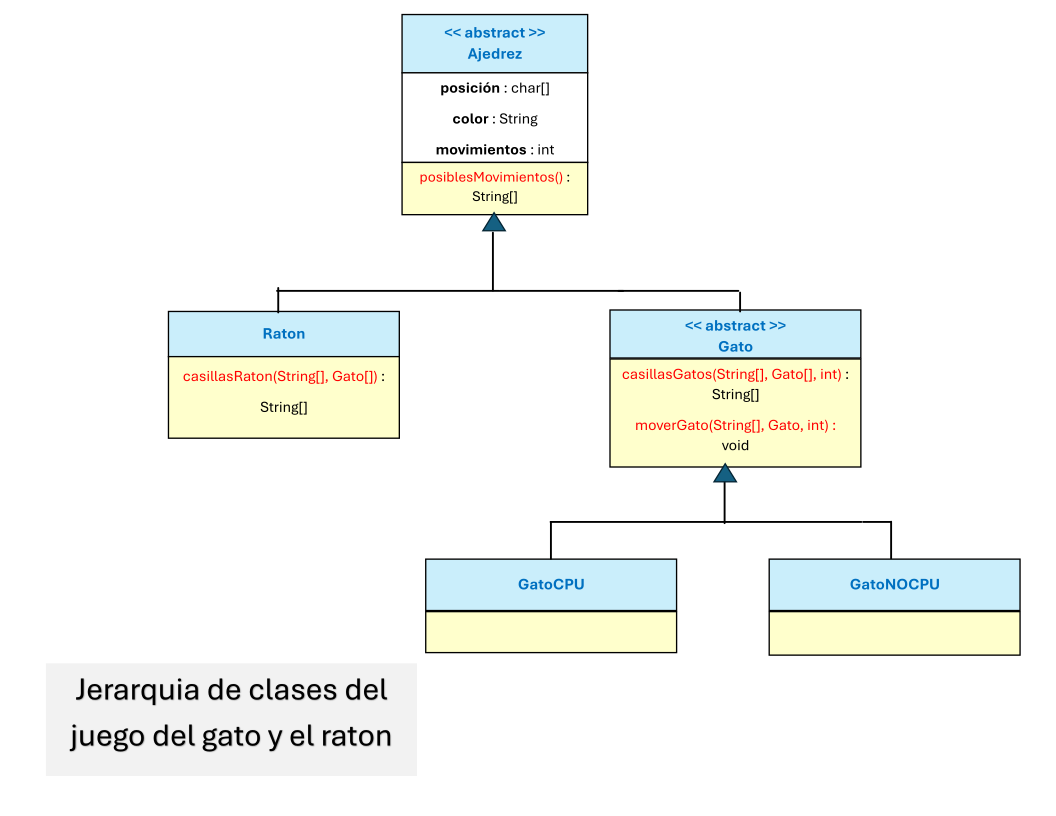
\includegraphics[scale=0.6]{gatoRaton.png}
	\end{figure}
	
	\section*{Descripción de proyecto y explicación del Diagrama UML} El juego del Raton y los gatos es un juego de 2 jugadores que se realiza en un tablero de ajedrez (donde el jugador que controla a los Gatos puede ser la CPU). Se usan cinco fichas, una de color blanco que representa el ratón y cuatro fichas negras para representar a los gatos. Tanto el ratón como los gatos se mueven en diagonal, siempre por las casillas negras. Los gatos no pueden retroceder, mientras que el ratón sí puede hacerlo (siempre en diagonal). Al comienzo de la partida los gatos se colocan en las casillas negras de la última fila del tablero, y el ratón en una de las casillas negras de la primera fila. El objetivo del ratón es llegar a la última fila del tablero y el de los gatos acorralar al ratón, hasta dejarlo sin poder realizar movimiento alguno. El jugador que tiene el ratón gana si llega a la orilla opuesta del tablero, y el jugador que tiene a los gatos gana si el ratón no puede realizar movimiento alguno porque los gatos lo acorrallaron.
	
	En el diagrama tenemos la clase abstracta Ajedrez que representa el comportamiento de las fichas en el juego, es decir, los movimientos del Gato y al Ratón sobre el tablero.
	Todas las fichas tienen asociada una posición dentro del tablero, su color para determinar si son un gato o un ratón, y la cantidad de movimientos que pueden hacer en función de su posición (como un valor numérico)
	
	De todas las fichas podemos conocer la lista de casillas a las que se pueden mover según su posición en el tablero (es decir, sus posibles movimientos), usando el metodo abstracto posiblesMovimientos() que revisa los movimientos que puede hacer la ficha y dice a que posiciones se puede mover (guardandolas en una lista y retornando esa lista con posibles movimientos)
	
	Para los gatos, como particularmente no pueden retroceder y ademas pueden ser una computadora, definimos además el método de moverGato() como método abstracto para aplicar polimorfismo al movimiento de los gatos (porque un gato usuario es distinto de un gato computadora). También, como es claro que los gatos pueden estorbarse entre sí, definimos además un método casillasGatos() que obtiene los VERDADEROS posibles movimientos de los gatos, usando como parametros: 
	\begin{itemize}
		\item El arreglo de posibles movimientos al que vamos a estar modificando para que únicamente se quede con los movimientos posibles.
		\item El arreglo que tiene la posición de los 4 gatos.
		\item El gato que estamos revisando de los 4, (créeme, este parametro es importante.)
	\end{itemize}
	Y retorna el arreglo con las casillas que puede tocar el gato.
	
	Por supuesto, como hacemos la distinción entre un gato controlado por una computadora y un gato que no es controlado por una computadora. Incluimos a las subclases GatoCPU y GatoNOCPU para implementar dentro de esas clases el metodo de moverGato() especifico para un GatoCPU y un GatoNOCPU.
	
	Finalmente, como al ratón siempre lo controla un humano, únicamente definimos el metodo moverRatón() que es análogo al de moverGato(), es decir, devuelve la lista de los verdaderos posibles movimientos de un ratón a partir de la lista entregada por el método posiblesMovimientos() y las posiciones de los gatos 4 gatos (pues es claro que un gato puede estorbarle a un ratón).
	
	Al finalizar cada partida, vamos a guardar un registro con las siguientes columnas:
	\begin{itemize}
		\item Los movimientos del ratón durante la partida
		\item Los movimientos del gato durante la partida
		\item El resultado del juego (es decir, si ganó el ratón o si ganaron los gatos).
	\end{itemize}
	
	Dichos registros se guardan en un sistema de archivos y esperamos encontrar intersecciones entre los conjuntos de movimientos del ratón en los diferentes archivos, para lograr los objetivos del proyecto. 
\end{document}
